\documentclass{article}
\usepackage[T1]{fontenc}
\usepackage[utf8]{inputenc}
\usepackage[french]{babel}
\usepackage{url}
\usepackage{hyperref}
\usepackage{amsfonts}
\usepackage{amsmath}
\usepackage{amsthm}
%\usepackage{titling}
%\usepackage{pdfpages}
\usepackage[left=3cm,right=3cm]{geometry}
\usepackage{graphicx}
\usepackage{float}

%\setlength{\droptitle}{-10em}

\renewcommand{\thesection}{\Roman{section}}
\renewcommand{\thesubsection}{\thesection.\arabic{subsection}}

\newcommand{\cont}{\mathcal{C}^0}
\newcommand{\cun}{\mathcal{C}^1}
\newcommand{\cinf}{\mathcal{C}^\infty}
\newcommand{\R}{\mathbb{R}}
\newcommand{\N}{\mathbb{N}}

\newtheorem{thm}{Théorème}
\newtheorem{lemm}{Lemme}
\theoremstyle{definition}
\newtheorem{defn}{Définition}
\begin{document}

%\includepdf{pagedegarde.pdf}

\setcounter{page}{1}

\title{Théorie des catastrophes}
\author{Farid Arthaud}
\date{\today}
\maketitle

\section{Introduction}

La théorie des catastrophes est l'étude de variations soudaines -- ou discontinuités -- naissant de perturbations continues. Elle découle intuitivement de questionnements physiques, notamment du comportement de certains systèmes physiques comme le roulis d'un navire ou le flambage d'une poutre.

La théorie des catastrophes est née dans les années 60, quasiment entièrement du travail de René \textsc{Thom} puis de Christopher \textsc{Zeeman}.
Dans son livre \textit{Stabilité structurelle et morphogenèse}, le \textit{théorème de classification de \textsc{Thom}} est établi: les singularités des applications à images dans un espace de dimension au plus cinq peuvent être classifiées en sept catégories.
Il s'agit du pli, de la fronce, la queue d'aronde, la vague, le poil, le papillon et le champignon.
Malgré les noms fantaisistes, il s'agit de catégories précises qui comprennent l'arité des fonctions et leur forme au voisinage de la singularité, à un changement de coordonnées près.

Une des applications principales de cette théorie sont les simulations: de phénomènes physiques mais aussi sociaux (comportements durant des révoltes, ...) et économiques.
Son utilité pour la physique découle de ce que \textsc{Demazure} appelle `\textit{la philosophie de la théorie des catastrophes}': l'étude de fonctions de classe infinie peut être vue comme celle d'une fonction potentiel définie sur l'espace des états possibles d'un système physique.
On s'intéresse dès lors aux états d'équilibre dudit système, et de leur stabilité; ce qui est précieux pour le physicien.

Cependant, nombre de ses applications sont controversées, notamment celles qui essaient d'expliquer un comportement humain par des mathématiques, pour des raisons éthiques, ou du manque de pertinence d'une telle comparaison.

\section{Catastrophes}

\subsection{Points critiques, variétés}

Soit $f:E\to F$, de classe $\cun$.
\begin{defn}
	Un point critique pour $f$ est un point $a$ où $df_a$ n'est pas surjective.

	Un point critique $a$ est dit non dégénéré si le déterminant Hessien de $f$ en $a$ est non nul.
\end{defn}

La théorie des catastrophes s'intéresse aux points critiques d'une fonction -- mais pas n'importe laquelle.
Il s'agit de travailler avec des fonctions définies sur des \textbf{sous-variétés}, qui sont la généralisation de courbes et surfaces aux dimensions supérieures.
\begin{defn}
	Une \textbf{sous-variété} $V$ de $\R^n$ est un ensemble qui est localement descriptible par un \textbf{système non dégénéré d'équations locales}.
	Cela signifie qu'il existe pour tout point $a\in V$ un voisinage $U$ et $\Phi_1,...,\Phi_m: U \to\R$ telles que $U\cap\{x\mid \Phi_1(x)=...=\Phi_m(x)=0\}=U\cap V$; et que $d\Phi_{1,x},...,d\Phi_{m,x}$ forment un système libre de formes linéaires.

	L'entier $m$ s'appelle la codimension de la sous-variété, que l'on suppose être la même en tout point de $V$ par la suite (on peut supposer la variété connexe par exemple).
\end{defn}
\begin{thm}
	Une variété de dimension $p$ admet en tout point un espace tangent de dimension $p$.
	C'est en fait l'intersection des noyaux du système d'équations locales définissant $V$ en ce point.
\end{thm}

Une application définie sur un ensemble quelconque est dite de classe $\cinf$ si elle peut être prolongée en une fonction $\cinf$ sur un ouvert contenant cet ensemble. Soit $V$ une sous-variété et $F$ un espace vectoriel.
\begin{defn}
	$f$ est un \textbf{plongement} si $f(V)$ est une sous-variété de $F$ et $f$ induit un ($\cinf$-) difféomorphisme $V\to f(V)$.
\end{defn}

Ces notions nous permettent d'établir un cadre à l'étude de fonctions allant d'une variété vers une autre.

\subsection{Transversalité et généricité}

La \textbf{transversalité} est une hypothèse sur l'intersection de deux objets permettant d'affirmer qu'elle est `non particulière' -- c'est ce que l'on pourrait abusivement appeller un ``positionnement général'', ce que l'on verra à travers les \textit{théorèmes de transversalité}.
\begin{defn}
	Deux sous-espaces vectoriels de $\R^n$ $F$ et $G$ sont dit \textbf{transverses} si $F+G=\R^n$.
\end{defn}

On trouve en annexe des exemples d'intersections transverses et non transverses.

Une première condition de transversalité est: $F$ et $G$ sont transverses si et seulement si $dim(F\cap G)\leq dim(F)+dim(G)-n$ ou encore $codim(F\cap G)\geq codim(F)+codim(G)$.
On constate que si la somme des dimensions est strictement inférieure à $n$, les espaces ne peuvent être transverses: la transversalité dépend fortement de l'espace dans lequel on travaille.

Une autre condition de transversalité, cette fois-ci géométrique, est que tous espaces affines parallèles à $F$ et $G$ soient d'intersection non vide.
Si la somme des dimensions vaut au moins $n$, une condition de transversalité est que l'intersection soit de dimension minimale.

On généralise ensuite la définition à deux variétés: elles sont transverses si leurs plans tangents sont transverses en tout point de leur intersection.
Puisque les espaces tangents de la variété sont de même dimension que la variété, la somme des dimensions des variétés doit valoir au moins $n$ pour qu'elles soient transverses (aux points où elles s'intersectent).

On remarque de plus qu'une intersection transverse de sous-variétés est une sous-variété, puisque l'espace tangent est justement l'intersection des noyaux des différentielles des coordonnées locales, et que la concaténation des systèmes de coordonnées locales en forme un si et seulement si cette intersection forme un espace de dimension minimale.

La transversalité est donc une condition forte permettant de `repérer' une sous-variété, comme vu pour une intersection mais aussi pour une image:
\begin{thm}
	Soient $V$ et $W$ deux variétés, $U$ un ouvert contenant $V$ et $f:U\to W$ de classe $\cinf$.
	Si $a\in V$, $f(a)\in W$ et l'image de l'espace tangent à $V$ en $a$ par $df_a$ est transverse à l'espace tangent à $W$ en $f(a)$, alors $V\cap f^{-1}(W)$ est une sous-variété en $a$ de codimension $codim_a(V) + codim_{f(a)}(W)$.
\end{thm}

La version faible du théorème de transversalité s'énonce à partir d'une fonction $f: \Lambda\times V\to F$ de classe $\cinf$, où $\Lambda\in G$ est un ouvert d'un espace normé servant à `indexer' une famille de fonctions $V\to F$.
\begin{thm}[de transversalité faible]
	Si $f$ est transverse à $W$, une sous-variété de $F$, alors l'ensemble des $\lambda\in\Lambda$ tels que $x\mapsto f(x,\lambda)$ soit transverse à $W$ est dense dans $\Lambda$ en tant qu'intersection dénombrable d'ouverts denses.
\end{thm}

Ainsi, étant donnée une famille de fonctions $f_\lambda: V\to F$ avec des hypothèses de régularité sur la dépendance en $V$ et en $\Lambda$, on peut affirmer que l'on peut approcher un $f_\lambda$ arbitrairement bien par des applications $f_{\lambda'}$ transverses à $W$.

La transversalité est donc un `positionnement générique', dans le sens de la densité.
On verra une version plus forte de ce théorème lors de l'étude du théorème de classification de \textsc{Thom}.

\subsection{Réecriture au voisinage d'un point critique}

La classification des points critiques demande une forme d'équivalence permettant de mettre les fonctions dans une forme commune au voisinage du point critique, les rendant comparables.
On a pour cela à notre disposition un certain nombre de lemmes et théorèmes permettant des réecritures semblables.

Pour cela, on introduit une relation d'équivalence sur les couples $(a,f)$ où $f\in\cinf(U_f,F_f)$: $(a,f)$ et $(b,g)$ sont en relation si et seulement s'il existe un difféomorphisme $u$ d'un voisinage de $b$ vers un voisinage de $a$ tel que $(f-f(a))\circ u = (g-g(b))$.

Cette équivalence permet donc de mettre en relation des applications au voisinage d'un point ``à un système de coordonnées locales près''.

Par exemple, dans le cas de la dimension $1$, $\R\to\R$, si $f(0)=f'(0)=...=f^{(k-1)}=0$ et $f^{(k)}(0)\neq 0$ alors, il existe un voisinage de 0 et un changement de coordonnées dans lesquelles $f(x)=\pm x^k$ (qui est d'ailleurs un $+$ si $k$ est impair).

Deux fonctions sont en relation si et seulement si leurs écritures en ces coordonnées $\pm x^k$ et $\pm x^l$ ont le même signe et indice ($k=l$). Ceci fournit une classification des points critiques en dimension 1, en fonction de leurs dérivées successives.

Tout d'abord vient le fameux \textbf{théorème d'inversion locale}, qui permet de traiter les points non critiques d'une fonction. Soit $U$ un ouvert d'un espace vectoriel.
\begin{thm}[d'inversion locale]
	Si $f\in\cinf(U,\R^m)$, et que $df_a$ est bijective, alors f est un difféomorphisme local: elle est bijective d'un voisinage de $a$ vers un voisinage de $f(a)$, de réciproque $\cinf$.

	On en déduit qu'au voisinage de $a$, il existe un système de coordonnées locales telles que $f(x)=f(a)+x$, ou encore que $(a,f)$ est équivalent à $(0,Id)$.
\end{thm}
\begin{proof} Voir annexe. \end{proof}

Ce théorème est équivalent à celui des \textit{fonctions implicites}, dont on trouve l'énoncé en annexe.
Le \textbf{lemme d'\textsc{Hadamard}} permet de faire intervenir les coordonnées de $f$ dans son écriture au voisinage de $0$, nous permettant de nous rapprocher d'une écriture standard.
\begin{lemm}[d'\textsc{Hadamard}]
	Si $f\in\cinf(U,\R)$ s'annule en $0$, alors il existe un voisinage de $0$ sur lequel $f$ peut s'écrire: $f(x)=x_1g_1(x)+...+x_ng_n(x)$ avec $g_i\in\cinf$ et $g_i(0) = \frac{\partial f}{\partial x_i}(0)$.

	Si 0 est point critique, on peut réitérer cela et écrire (toujours sur un voisinage de 0):
	$$f(x)=\sum_{1\leq i,j \leq n} x_ix_jh_{ij}(x)$$
\end{lemm}
\begin{proof} Voir annexe. \end{proof}

Ce dernier lemme permet de démontrer le \textbf{lemme de \textsc{Morse}}, qui donne une expression nettement plus simple au voisinage d'un point critique à condition qu'il soit non dégénéré.
\begin{lemm}[de \textsc{Morse}]
	Si $f\in\cinf(\R^n,\R)$ admet un point critique non dégénéré en $u$, alors il existe un voisinage de $u$ et un $\cinf$-difféomorphisme $y=(y_1,...,y_n)$ tel que:
	$$f=f(u)+y_1^2+...+y_l^2-y_{l+1}^2-...-y_n^2$$
\end{lemm}
\begin{proof} Voir annexe. \end{proof}
\begin{defn}
	Une application de la forme $(y_1,...,y_n)\mapsto a+y_1^2+...+y_k^2-y_{k+1}^2-...-y_n^2$ est appelée \textit{k-saddle de \textsc{Morse}}.
\end{defn}

De plus, on note que si $f$ est \textit{0-saddle} alors $u$ est minimum local, et si $f$ est \textit{n-saddle}, alors $u$ est maximum local.
Si $f$ est $k-saddle$ de \textsc{Morse} en $u$, c'est un point critique isolé, et puisqu'un changement de coordonnées conserve l'isolation, on en déduit que tout point critique non dégénéré est isolé.
De plus, l'indice $k$ est invariant par changement de coordonnées, c'est une propriété intrinsèque à $f$ (ou plutôt à sa forme Hessienne).

Vient enfin le \textbf{théorème de décomposition}, qui permet de traiter les cas où le point critique est dégénéré en appliquant le théorème de \textsc{Morse} à une partie des coordonnées de $f$.
\begin{thm}[de décomposition]
	Si f admet 0 pour point critique et $H(f)_0$ est de rang $r$, alors $f$ est équivalente (au sens défini ci-dessus) au voisinage de 0 à une fonction de la forme:
	$$g(x)= x_1^2+x_2^2+ ...+x_p^2-x_{p+1}^2 -...- x_r^2 + h(x_{r+1},...,x_n)$$
	où $h\in\cinf$ telle que $dh(0)=0$ et $d^2h(0)=0$.
\end{thm}

\subsection{Jets et espace des germes}
\begin{defn}
	Le \textit{k-jet} de $f$ en $x$ est le $(k+1)$-uplet associé aux $k$ premières différentielles successives de de $f$ en $x$: $j^k_x f = \left(f(x), df_x, ..., d^kf_x\right)$.

	Le $r$-germe de $f$ en un point associé à $k\in\N^*$ est le couple $(x,j^k_x f)$. On note $J^r(U,F)$ l'\textbf{espace des germes d'odre r}.
\end{defn}

L'espace des germes permet d'exprimer des relations entre les dérivées partielles des fonctions (à un choix de coordonnées près) par exemple, et son couplage avec la notion de transversalité fournit des résultats puissants.

On aboutit enfin au \textbf{théorème de transversalité \textsc{Thom}}, qui est l'outil principal de la classification des \textit{applications génériques} (c'est à dire qui appartiennent à une réunion d'ouverts denses).
\begin{thm}[de transversalité de \textsc{Thom}]
	L'ensemble des $f\in\cinf(U,F)$ telles que $j^rf$ soit transverse à une sous-variété donnée de l'espace des germes $J^r(E,F)$ est une partie dense.
\end{thm}

\section{Classification des catastrophes}
\subsection{Surfaces de $\R^3$}

On prend $f: \R^3\to\R$ de classe $\cinf$, et on s'intéresse à l'ensemble de $\R^3$ défini par $V=\{x\mid f(x)=0\}$.
Il est clair qu'on ne peut rien dire dans le cas général, puisque $V$ peut alors être quelconque (en particulier, tout sous-espace vectoriel est envisageable).

Cependant, lorsqu'on impose que $f$ soit générique, il devient possible de commenter la forme de $V$.
Spécifiquement, on s'intéresse à la projection de $V$ sur le plan $(x,y)$.

Un point où $\frac{\partial f}{\partial z}\neq 0$ se manifeste par le fait que cette projection est un simple changement de coordonnées locales: c'est le théorème des \textit{fonctions implicites}.
Il reste donc à traiter le cas des points où cette dérivée partielle s'annule, qui sont des points critiques particuliers de $f$.
On appelle \textit{contour apparent} l'ensemble des points où $f(x,y,z)=0$ et $\frac{\partial f}{\partial z}(x,y,z)=0$, cette notion est illustrée en annexe.
\begin{defn}
	$a$ est un \textbf{point-pli} s'il existe des coordonnées locales dans lesquelles
	$$\pm f(x, y, z) = z^2 - y$$

	$a$ est un \textbf{point-fronce} s'il existe des coordonnées locales dans lesquelles
	$$f(x,y,z) = z^3 - xz - y$$
\end{defn}
\begin{thm}
	Pour $f$ générique:
	\begin{enumerate}
		\item $\{f=0\}$ est une sous-variété de dimension deux (ou une \textbf{surface})
		\item Son contour apparent $\{f=0\}\cap \{\frac{\partial f}{\partial z}=0\}$ est une sous-variété de dimension un (ou une \textbf{courbe})
		\item Tous les points critiques sont des points-plis ou points-fronces, et les points-fronces sont isolés
	\end{enumerate}
\end{thm}
\begin{proof}[Démonstration (deux premiers points)] Voir annexe. \end{proof}

On obtient donc une classification des points de $V$: étant partis d'un ensemble pouvant être quelconque, on s'est ramenés au cas intuitif d'une surface dans $\R^3$ ayant un contour naturel lorsqu'elle est vue depuis une direction particulière.

\subsection{La machine à catastrophes de \textsc{Zeeman}}
Cette expérience classique, imaginée par Cristopher \textsc{Zeeman}, permet d'illustrer ce théorème dans un cas particulier.
On imagine un disque tournant sans frottement autour de son axe, ayant un point d'attache relié par deux élastiques à un point fixe (ou point d'ancrage) et à un point de contrôle que le manipulateur peut déplacer librement.
Les notations sont illustrées ci-dessous.

\begin{figure}[H]\centering 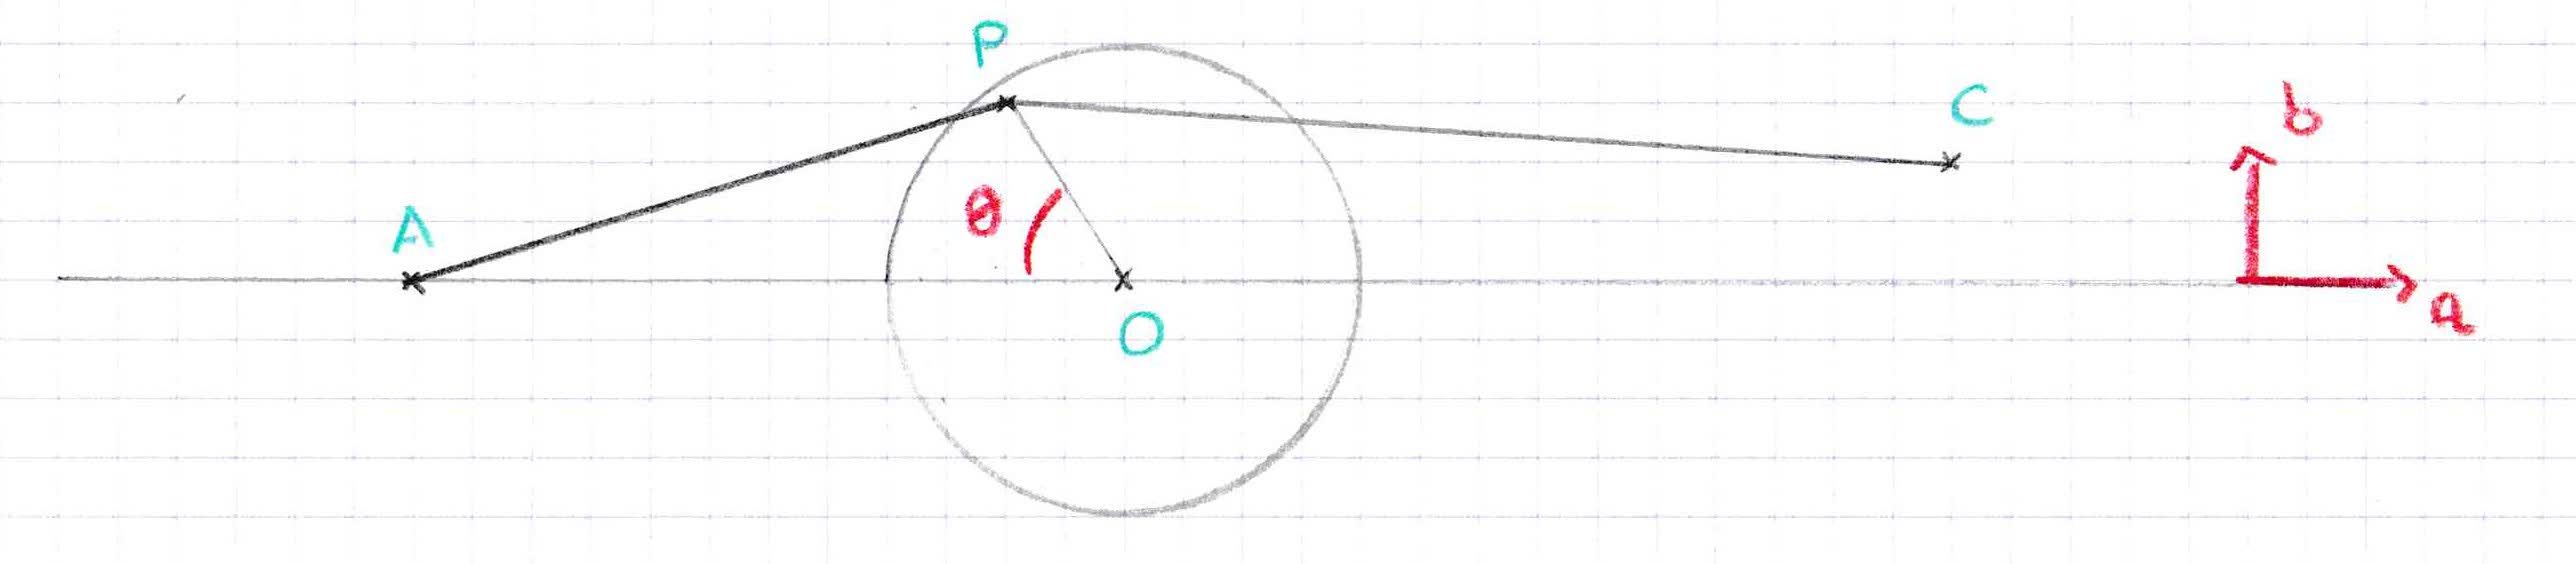
\includegraphics[width=10cm, keepaspectratio]{images/zeeman_sketch.jpg}\caption{Illustration de la machine de \textsc{Zeeman}}\end{figure}

On observe que pour certaines positions de contrôle, un léger déplacement du point de contrôle donne des variations soudaines de l'angle $\theta$ -- un ``saut'' du disque.

%\includepdf{annexe.pdf}

\end{document}

%%%%%%%
\begin{defn}
	Une application $f$ est dite \textbf{structurellement stable} si pour toute application $p$ suffisament proche de 0 (et infiniment continue), $f+p$ a le même type de point critique que $f$ à translation près.
\end{defn}

Un point critique est en fait structurellement stable si et seulement si il est non dégénéré.
La \textbf{stabilité structurelle} signifie plus généralement que le comportement qualitatif ne change pas malgré une perturbation suffisament petite.


Ces deux théorèmes, dont les énoncés généraux sont admis, permettent de ...
\begin{thm}[de \textsc{Whitney}]
	Si $V$ est une variété compacte de dimension $n$, il existe un plongement de $V$ dans $\R^{2n+1}$.
\end{thm}
\begin{thm}[de \textsc{Sard}]
	Si $f: U\to F$ où $U$ est un ouvert de $E$ est de classe $\cinf$ alors l'ensemble des images de ses points critiques est négligeable dans $F$.
\end{thm}
\begin{proof}{($E=F=\R$)} Voir annexe. \end{proof}

Sous sa forme géométrique, ce théorème dit que ...

\subsection{Théorème de \textsc{Whitney}}

On traite ici le cas des points critiques d'une application $\R^2\to\R^2$, où l'on obtient un résultat analogue au précédent.
Au voisinage d'un point ordinaire (non critique), il existe des coordonnées $(x',y')$ en $f(a)$ dans lesquelles $x' = x, y' = y$ (à l'aide du théorème \textit{inversion locale}), on définit donc encore deux `points-types' pour classifier les points critiques.
\begin{defn}
	$a$ est un \textbf{point-pli} s'il existe des coordonnées $(x',y')$ en $f(a)$ dans lesquelles $x' = x, y' = y^2$.

	$a$ est un \textbf{point-fronce} s'il existe des coordonnées $(x',y')$ en $f(a)$ dans lesquelles $x' = x, y' = y^3 - xy$.
\end{defn}
\begin{thm}[de \textsc{Whitney}]
	Une application générique $\R^2\to\R^2$ a ses points critiques le long d'une courbe composée de plis et de fronces, et les fronces sont des points isolés de cette courbe.
\end{thm}
